\documentclass[11pt]{article}
\usepackage[T1]{fontenc}
\usepackage[utf8]{inputenc}
\usepackage{lmodern}
\usepackage[margin=1in]{geometry}
\usepackage{amsmath,amssymb,amsthm,booktabs,graphicx,array}
\usepackage[round,authoryear]{natbib}
\usepackage{setspace}
\usepackage[colorlinks=true,allcolors=blue]{hyperref}
\usepackage{caption}
\captionsetup{font=small,labelfont=bf}
\newtheorem{proposition}{Proposition}
\newtheorem{corollary}{Corollary}
\newcommand{\E}{\mathbb{E}}
\newcommand{\ind}{\mathbf{1}}
% Generated by code/build_exhibits.py; never edit manually.
\newcommand{\BaselineN}{1793}
\newcommand{\EndlineN}{1751}
\newcommand{\DietN}{1728}
\newcommand{\BlockN}{22}
\newcommand{\FamilyN}{204}
\newcommand{\GikuriroCost}{124.49}
\newcommand{\LargeCost}{517.44}
\newcommand{\UpperCost}{121.24}
\newcommand{\LargeCoverage}{24.1}
\newcommand{\UpperLargeShare}{0.82}
\newcommand{\JointCrit}{3.124}
\newcommand{\HetMinP}{0.600}
\newcommand{\UpperRetention}{3.11}
\newcommand{\UpperRetentionSE}{1.10}
\newcommand{\UpperRetentionHolmP}{0.026}
\newcommand{\LargeDietEstimate}{0.545}
\newcommand{\LargeDietSE}{0.134}
\newcommand{\LargeDietLo}{0.281}
\newcommand{\LargeDietHi}{0.808}
\newcommand{\LargeDietP}{$<0.001$}
\newcommand{\LargeDietSimLo}{0.126}
\newcommand{\LargeDietSimHi}{0.963}
\newcommand{\LargeDietJointP}{$<0.001$}
\newcommand{\LargeDietHolmP}{0.013}
\newcommand{\GikuriroDietEstimate}{0.255}
\newcommand{\GikuriroDietSE}{0.131}
\newcommand{\GikuriroDietLo}{-0.002}
\newcommand{\GikuriroDietHi}{0.513}
\newcommand{\GikuriroDietP}{0.052}
\newcommand{\GikuriroDietSimLo}{-0.153}
\newcommand{\GikuriroDietSimHi}{0.664}
\newcommand{\GikuriroDietJointP}{0.912}
\newcommand{\GikuriroDietHolmP}{1.000}
\newcommand{\ControlLargeDietEstimate}{0.124}
\newcommand{\ControlLargeDietSE}{0.119}
\newcommand{\ControlLargeDietLo}{-0.110}
\newcommand{\ControlLargeDietHi}{0.358}
\newcommand{\ControlLargeDietP}{0.296}
\newcommand{\ControlLargeDietSimLo}{-0.247}
\newcommand{\ControlLargeDietSimHi}{0.495}
\newcommand{\ControlLargeDietJointP}{1.000}
\newcommand{\ControlLargeDietHolmP}{1.000}
\newcommand{\UpperLargeDietEstimate}{-0.094}
\newcommand{\UpperLargeDietSE}{0.170}
\newcommand{\UpperLargeDietLo}{-0.429}
\newcommand{\UpperLargeDietHi}{0.240}
\newcommand{\UpperLargeDietP}{0.579}
\newcommand{\UpperLargeDietSimLo}{-0.625}
\newcommand{\UpperLargeDietSimHi}{0.436}
\newcommand{\UpperLargeDietJointP}{1.000}
\newcommand{\UpperLargeDietHolmP}{1.000}
\newcommand{\LowerLargeDietEstimate}{-0.127}
\newcommand{\LowerLargeDietSE}{0.162}
\newcommand{\LowerLargeDietLo}{-0.446}
\newcommand{\LowerLargeDietHi}{0.192}
\newcommand{\LowerLargeDietP}{0.434}
\newcommand{\LowerLargeDietSimLo}{-0.632}
\newcommand{\LowerLargeDietSimHi}{0.379}
\newcommand{\LowerLargeDietJointP}{1.000}
\newcommand{\LowerLargeDietHolmP}{1.000}
\newcommand{\LargeShortfallEstimate}{0.073}
\newcommand{\LargeShortfallSE}{0.016}
\newcommand{\LargeShortfallLo}{0.042}
\newcommand{\LargeShortfallHi}{0.104}
\newcommand{\LargeShortfallP}{$<0.001$}
\newcommand{\LargeShortfallSimLo}{0.024}
\newcommand{\LargeShortfallSimHi}{0.123}
\newcommand{\LargeShortfallJointP}{$<0.001$}
\newcommand{\LargeShortfallHolmP}{0.001}
\newcommand{\ControlLargeShortfallEstimate}{0.004}
\newcommand{\ControlLargeShortfallSE}{0.014}
\newcommand{\ControlLargeShortfallLo}{-0.024}
\newcommand{\ControlLargeShortfallHi}{0.032}
\newcommand{\ControlLargeShortfallP}{0.758}
\newcommand{\ControlLargeShortfallSimLo}{-0.040}
\newcommand{\ControlLargeShortfallSimHi}{0.049}
\newcommand{\ControlLargeShortfallJointP}{1.000}
\newcommand{\ControlLargeShortfallHolmP}{1.000}
\newcommand{\GikuriroSavingEstimate}{1.186}
\newcommand{\GikuriroSavingSE}{0.338}
\newcommand{\GikuriroSavingLo}{0.520}
\newcommand{\GikuriroSavingHi}{1.853}
\newcommand{\GikuriroSavingP}{$<0.001$}
\newcommand{\GikuriroSavingHolmP}{0.052}
\newcommand{\LargeAssetsEstimate}{0.780}
\newcommand{\LargeAssetsSE}{0.118}
\newcommand{\LargeAssetsLo}{0.548}
\newcommand{\LargeAssetsHi}{1.012}
\newcommand{\LargeAssetsP}{$<0.001$}
\newcommand{\LargeAssetsHolmP}{$<0.001$}
\newcommand{\UpperLargeBreakEven}{0.094}
\newcommand{\LargeDietBudgetGain}{0.131}
\newcommand{\ProviderSavingUpper}{3.25}

% Generated referee-revision numbers; never edit manually.
\newcommand{\IdentifiedDietN}{1730}
\newcommand{\PairFamilyN}{828}
\newcommand{\BoundFamilyN}{1656}
\newcommand{\GKFittedRegret}{0.237}
\newcommand{\GKObservedRegretUpper}{0.763}
\newcommand{\GKPopulationRegretUpper}{1.172}
\newcommand{\LowerLargeFittedRegret}{0.000}
\newcommand{\LowerLargeObservedRegretUpper}{0.588}
\newcommand{\LowerLargePopulationRegretUpper}{0.908}
\newcommand{\HajekControlLargeEstimate}{0.039}
\newcommand{\HajekControlLargeSimLo}{-0.310}
\newcommand{\HajekControlLargeSimHi}{0.387}
\newcommand{\HajekLowerLargeEstimate}{-0.237}
\newcommand{\HajekLowerLargeSimLo}{-0.690}
\newcommand{\HajekLowerLargeSimHi}{0.215}

\onehalfspacing
\setlength{\emergencystretch}{1em}
\title{You give them something to eat:\\Dietary Diversity, Coverage, and Catholic Aid in Rwanda}
\author{Diego Gonz\'alez-Gonz\'alez\thanks{Research draft, September 2026. This paper uses public data from an experiment conducted by Craig McIntosh and Andrew Zeitlin, with Innovations for Poverty Action and the implementing organizations. It does not report a new field experiment. Code and drafting assistance were provided by OpenAI Codex; the draft requires the author's review before journal submission. No institutional affiliation, funding, or endorsement is asserted. Replication materials: \url{https://github.com/dgonzalezgonzalez/you-give-them-something-to-eat}.}}
\date{September 30, 2026}
\begin{document}
\maketitle
\begin{abstract}
\noindent Which allocation of aid can a food-security organization defend when experimental outcomes are noisy and some diets are unobserved? I reanalyze the village-randomized evaluation of Catholic Relief Services' Gikuriro program in Rwanda. Cash benchmarks are lotteries over observed packages at the same expected provider budget. I use known block-assignment probabilities to construct coherent dietary distributions, retain information in incomplete food modules, and bound policy regret over the baseline eligible population. A mixture of lower and large cash has the highest fitted mean dietary diversity. Gikuriro's observed-sample deficit against it is \GKFittedRegret\ food groups. All nine candidate policies remain compatible with mean optimality under simultaneous inference. Allowing arbitrary missing diets, the 95 percent upper regret bounds are \GKPopulationRegretUpper\ groups for Gikuriro and \LowerLargePopulationRegretUpper\ for the fitted cash policy. Thus the trial does not certify a small-loss allocation, although a loose one-group tolerance can be met by the latter conditional on the stated cluster approximation and transport assumptions. A household saving model illustrates why current food access need not rank intertemporal utility. The paper extends existing cash benchmarking through distributional and selection-aware decision accounting; it introduces neither a new experiment nor a new identification strategy.
\end{abstract}
\noindent\textbf{Keywords:} food security; Catholic Relief Services; cash transfers; dietary diversity; treatment allocation.\\
\textbf{JEL codes:} C93, D61, I32, O12.
\newpage

\section{Introduction}

An organization trying to improve food security faces a choice over both what to provide and how many households to reach. A program that offers nutrition advice, agricultural support, and access to saving groups can serve an entire eligible population at a modest cost per household. A large cash transfer may deliver a more visible change in the diets of its recipients, while leaving fewer resources for everyone else. Comparing the average outcomes of recipients in those two programs does not answer the organization's budget question. The relevant comparison includes the households that a more expensive intervention leaves untreated.

I examine this distinction in the Gikuriro program in Rwanda, implemented by Catholic Relief Services (CRS) and SNV with support from USAID. Gikuriro combined nutrition and health activities, agricultural support, saving groups, and water, sanitation, and hygiene interventions. Its stated aim was to improve maternal and child nutrition. The experiment conducted by \citet{mcintosh2024} assigned 248 villages to Gikuriro, control, or one of four cash-transfer amounts delivered by GiveDirectly. It therefore offers a credible comparison of a Catholic organization's bundled intervention with transfers of different sizes in the same population. The title recalls Mark 6:37; the empirical question concerns the consequences of aid delivery, rather than a comparison of religious affiliations.

The original study develops equal-cost cash benchmarking and explicitly discusses cost effectiveness and the choice between coverage and intensity. The mean Gikuriro-versus-control/large contrast used here is exactly the difference between its two cost-effectiveness ratios, multiplied by Gikuriro's cost. It consequently has the same studentized statistic. I do not claim that coverage, convex mixtures, or this mean comparison is new. I use the corrected public data to ask what those comparisons support once the objective concerns a diet distribution, missing outcomes are allowed to differ across arms, and the organization must choose from several feasible allocations.

This change in the policy margin matters for distributional outcomes. An interpolated cash transfer could leave every household with some assistance. A coverage lottery leaves a fraction with the control outcome and gives the remainder the large package. Their means can agree even when their lower tails differ. I estimate treatment effects on the entire set of integer diet thresholds and on shortfall measures that put greater weight on diets with fewer food groups. I treat these measures as alternative priorities within a food-access objective. They are not monetary welfare measures, and the illustrative thresholds are not diagnostic cutoffs for hunger.

The experiment gives a precise estimate that large cash improves the diets of households living in assigned villages. The estimated gain is \LargeDietEstimate\ food groups, with a simultaneous confidence interval of [\LargeDietSimLo, \LargeDietSimHi]. Its cost per eligible household, however, is \$\LargeCost, compared with \$\GikuriroCost\ for Gikuriro. Financing large cash from that budget permits coverage of \LargeCoverage\ percent of villages. The estimated Gikuriro advantage over this lottery is \ControlLargeDietEstimate\ groups, with a simultaneous confidence interval spanning \ControlLargeDietSimLo\ to \ControlLargeDietSimHi. The data allow materially different rankings. They do not establish equivalence.

The fitted best cash policy combines lower and large transfers. It gives every village some cash, while reserving the large package for a minority. In the original ANCOVA specification, Gikuriro's mean contrast against this policy is \LowerLargeDietEstimate\ groups, with simultaneous interval [\LowerLargeDietSimLo, \LowerLargeDietSimHi]. A positive-weight estimator that adjusts explicitly for block assignment probabilities gives \HajekLowerLargeEstimate. The change in magnitude matters, but neither specification establishes the sign. The policy set, rather than the fitted winner alone, is therefore the object of inference.

Why might a nutrition program improve some economic outcomes without producing a clear dietary response within the observation period? I develop a household model in which food competes with saving for a limited current budget. Cash relaxes that budget, while access to a saving technology raises the return to resources carried forward. With background future income, the latter change can increase saving and intertemporal utility while reducing current food spending. Dietary variety responds at discrete food-purchase thresholds, so small changes in spending need not change the score. This mechanism is consistent with the original study's saving result and the substantial productive-asset response to large cash. It is not identified separately by the bundled intervention.

The economic literature gives several reasons to take this distinction seriously. \citet{curriegahvari2008} discuss paternalism, externalities, and interdependent preferences as rationales for in-kind provision. \citet{banerjeeduflo2007} show that poor households allocate resources across needs that extend beyond food. The randomized cash experiment of \citet{haushofer2016} measures changes in consumption and assets alongside food security. Those findings make a single current-diet outcome an incomplete criterion for overall aid effectiveness. \citet{egger2022} also demonstrate that cash can affect nonrecipients through the local economy, which limits policy extrapolations that hold spillovers fixed.

The policy-allocation problem is established in the work of \citet{manski2004} and \citet{kitagawa2018}. I evaluate a finite policy class and report confidence sets and regret bounds, including the uncertainty induced by selection. This adds decision accounting to the Rwanda evidence: a fitted optimum can coexist with a wide set of statistically admissible policies, and a narrow sample identification region can coexist with an uninformative population confidence region. The contribution is this empirical distributional reanalysis. Its economic value depends on the loss an organization can tolerate; a precise winning allocation is not established by the available data. Local prices further limit scale extrapolation, as the cash-versus-food experiment of \citet{cunha2019} demonstrates.

\section{A framework for nutrition, saving, and coverage}

\subsection{Household allocation}

A household has current resources $w+t$, where $w$ is its initial budget and $t$ is a transfer. It allocates resources to current food expenditure $f$ and saving $s$. Food is measured in units with price normalized to one. Let $\underline f$ denote subsistence expenditure, $R$ the positive gross return on saving, $y>0$ background future income, and $\beta>0$ the weight on future consumption. For an interior household with $w+t>\underline f$, preferences and the budget constraint are
\begin{equation}
 U(f,s)=\log(f-\underline f)+\beta\log(Rs+y),\qquad
 f+s=w+t,\quad s\geq0. \label{eq:household}
\end{equation}
The future resource $y$ is important: it allows a change in the saving return to affect the allocation between dates. The model abstracts from risk, credit, household bargaining, and the multiple activities provided by Gikuriro. Its comparative statics describe a possible mechanism within that bundle.

Food diversity is an increasing step function of spending,
\begin{equation}
 D(f)=\sum_{j=1}^{12}\ind\{f\geq a_j\}, \qquad
 \underline f\leq a_1\leq\cdots\leq a_{12}, \label{eq:diet}
\end{equation}
where $a_j$ are household-specific thresholds for including additional food groups. This reduced form allows a household to maintain a staple diet while deferring more expensive sources of variety. It does not imply that each food group has the same nutrient content or that variety depends only on total expenditure.

\begin{proposition}[Current food and saving]
If the optimum is interior, then
\[
 f^*=\frac{w+t+y/R+\beta\underline f}{1+\beta},\qquad
 s^*=\frac{\beta(w+t-\underline f)-y/R}{1+\beta}.
\]
Cash increases both current food expenditure and saving. A rise in $R$ decreases current food expenditure, increases saving, and increases maximized household utility. Dietary diversity weakly increases with cash, but can remain unchanged over an interval of transfer values.
\end{proposition}

If saving is constrained at zero, a small change in its return has no effect on allocation; cash initially finances current spending. The saving-return prediction holds $y$ fixed. I do not estimate $R$, $y$, or $\beta$: saving groups may change fees, credit, risk or commitments instead. The model illustrates how current food access and intertemporal utility can rank an intervention differently.

\begin{corollary}[A short observation window]
A saving intervention can raise household utility while leaving the observed diversity score unchanged, or reducing it. A small cash transfer can raise food spending without increasing the diversity score. A larger transfer crosses a threshold only if an uncrossed threshold is reachable; a household already consuming all twelve groups cannot increase this score.
\end{corollary}

The bundled assignment cannot distinguish this channel from delivery timing or other program components. Repeated measurements or randomized mechanism variation would be needed.

\subsection{The organization's budget}

Let $a\in\mathcal A=\{0,g,\ell,m,u,L\}$ denote control, Gikuriro, and the four cash packages. Each package has provider cost $c_a$ per eligible household, with $c_0=0$. Let $D_i(a)$ be household $i$'s diet under assignment of its village to package $a$. For a specified diet objective $v$, define $\mu_a(v)=\E[v(D_i(a))]$ in the baseline eligible population. Examples include $v(d)=d$ and
\begin{equation}
 v_{z,r}(d)=-\left(\frac{(z-d)_+}{z}\right)^r,
 \qquad z>0,\ r\in\{1,2\}. \label{eq:shortfall}
\end{equation}
Here $(x)_+=\max(x,0)$. A higher value denotes a smaller diet shortfall. The $r=2$ objective gives extra weight to a reduction among households further below the threshold. This adapts the shortfall structure of \citet{foster1984} to a diet proxy; it does not define an official poverty or nutrition line.

A policy chooses village-assignment probabilities $q_a\geq0$ with $\sum_aq_a=1$. The probabilities are independent of potential outcomes within the target blocks. At expected budget $b$, the organization faces
\begin{equation}
 \max_{q}\sum_aq_a\mu_a(v)
 \quad\text{subject to}\quad \sum_aq_ac_a\leq b. \label{eq:planner}
\end{equation}
This is an expected-cost constraint per eligible household. It is not an exact realized spending cap for a finite set of differently sized villages. Whole-village lotteries preserve the treatment saturation and within-village spillovers of each experimental arm; individual-level selective targeting is outside this policy class.

\begin{proposition}[Observed-package benchmarks]
Under stable package delivery, fixed costs per eligible household, and no cross-village interference, a village lottery has distribution
\[
 F_q(d)=\sum_aq_a F_a(d)
\]
and objective $\mu_q(v)=\sum_aq_a\mu_a(v)$. A solution to \eqref{eq:planner} exists with at most two packages in its support. If one package alone is feasible and exhausts no more than the budget, it may also be optimal.
\end{proposition}

Thus a cash-only benchmark at $b=c_g$ can be constructed from a finite list. It includes each pure cash arm costing no more than $c_g$ and each pair of packages whose costs bracket $c_g$. For $c_a<c_g<c_b$, the weight on the expensive package is
\begin{equation}
 q_b=\frac{c_g-c_a}{c_b-c_a},\qquad q_a=1-q_b. \label{eq:mix}
\end{equation}
Leaving part of the budget unspent is feasible in \eqref{eq:planner}. Spending it on an unobserved larger transfer would require an additional response assumption.

\begin{corollary}[Coverage versus intensity]
The large-cash/control lottery uses $q_L=c_g/c_L$. Universal Gikuriro has the higher value for objective $v$ if and only if
\[
 \mu_g(v)-\mu_0(v)\ \geq\ \frac{c_g}{c_L}\,[\mu_L(v)-\mu_0(v)].
\]
The ordering of package assignment effects alone is insufficient for this comparison.
\end{corollary}

For the mean objective, the left-minus-right treatment contrast is
$c_g\{\tau_g/c_g-\tau_L/c_L\}$. This is the original cost-effectiveness comparison expressed in food groups per eligible household. No additional identifying information is created by rescaling it.

The conditional assumptions matter economically. Cash prices or saving-group returns can change when the share of treated villages changes. Program overhead need not scale proportionally with the number of eligible households. An organization that cannot use lotteries, must provide universal minimum assistance, or values the geographic continuity of services faces a different feasible set. The trial identifies outcomes under its observed assignments. It does not identify arbitrary changes in saturation or delivery scale.

\subsection{Distributional priorities and unmeasured benefits}

If a policy improves all survival probabilities $\Pr(D\geq k)$, it improves every increasing function of the bounded integer score. If it improves all negative shortfalls $-\E[(z-D)_+]$, it is preferred by increasing concave functions of that score. These comparisons summarize priorities over the measured diet distribution. They require coherent population distributions and credible inference across thresholds. An estimated sign at one threshold is not sufficient to establish dominance.

A broader charity objective could also place value on future consumption, health, or public services. Write $\widetilde\mu_a=\mu_a(v)+H_a$, where $H_a$ is the value of all omitted consequences in the same units as the diet objective. If $\Delta_{gq}(v)=\mu_g(v)-\mu_q(v)$, Gikuriro is preferred when
\begin{equation}
 H_g-H_q\geq-\Delta_{gq}(v). \label{eq:breakeven}
\end{equation}
This inequality defines a break-even accounting requirement. It does not estimate $H_g$, monetize saving, or establish social welfare. Its empirical use is to show how much unmeasured value a particular diet comparison would need to overturn a ranking, along with the uncertainty in that requirement.

\subsection{Choice under uncertainty}

For the nine candidate policies, define regret in the measured objective as
$\mathcal R(a)=\max_b\{\mu_b(v)-\mu_a(v)\}$. A policy's fitted regret is the difference from the fitted best candidate. It is not its population opportunity cost. Suppose simultaneous inference supplies $L_{ba}\leq\mu_b-\mu_a\leq U_{ba}$ for every ordered pair, including $L_{aa}=U_{aa}=0$.
\begin{proposition}[Policy sets and regret accounting]
On the joint coverage event,
\[
 \max_b L_{ba}\leq\mathcal R(a)\leq\max_b U_{ba}.
\]
Every optimal policy belongs to the set $\{a:\max_b L_{ba}\leq0\}$. A policy with $\max_b U_{ba}\leq\epsilon$ has regret no greater than tolerance $\epsilon$ on that event.
\end{proposition}
The proposition is an elementary consequence of simultaneous inequalities, not a new treatment-choice result. Its usefulness here is to expose the decision content of the experiment. For interval outcomes, an upper bound on each pairwise upper endpoint also bounds regret uniformly over the admissible missing diets. A zero lower regret bound does not establish that a policy is optimal. A tolerance must come from the organization's objective; the quarter-, half-, and one-group values below are illustrative decision scenarios, not estimated donor preferences.

\section{Setting and data}

\subsection{Interventions and the experiment}

The baseline survey took place in August and September 2016 and the endline in September and October 2017. CRS and SNV implemented Gikuriro through local partners. Its activities included village nutrition schools, farmer field learning schools, support for small livestock and agricultural inputs, Savings and Internal Lending Communities, and environmental health promotion. Eligibility combined poverty classification and the presence of a young child or a pregnant or lactating woman. I retain the study's IPA-defined baseline eligible population rather than selecting households by actual receipt.

The trial assigned 74 villages to Gikuriro, 74 to control, and 100 to cash. The cash villages were split into three smaller arms of 22 villages each and a large arm of 34 villages. Randomization was blocked; the released data contain \BlockN\ blocks. Cash payment modality also varied within the cash villages. I average over the modality mix as implemented in each village-level package. These estimates do not describe an independently selected payment schedule.

Every block contains one lower, one middle, and one upper cash village, one or two large-cash villages, and three or four villages in each of control and Gikuriro. Block sizes range from ten to thirteen. The replication file \texttt{assignment\_probabilities.csv} gives all 132 block/arm cells and their known assignment probabilities. These probabilities are distinct from household survey weights. In the corrected release, each baseline eligible household's \texttt{samp\_wgt} equals its village's eligible frame count divided by the number sampled, within source floating-point precision. The weight is constant across rounds. The original paper mentions intensive-tracking adjustments, but this field does not contain a recoverable separate tracking factor. I therefore use the verified expansion weight and retain explicit observation bounds; I do not assert that an unavailable tracking adjustment makes attrition ignorable.

The cost comparison follows the original study's cost per eligible household, which incorporates observed compliance and provider accounting. For Gikuriro, \$\GikuriroCost\ differs from the cost per actual beneficiary because part of its overhead remains when an eligible household does not participate. The large-cash package costs \$\LargeCost\ per eligible household. These amounts are study-period US dollars, not contemporary program prices. I treat them as documented inputs rather than precisely estimated economic costs.

\begin{table}[t]
\centering\caption{Experimental arms, costs, and the eligible analysis population}\label{tab:design}
\resizebox{\textwidth}{!}{\begin{tabular}{lrrrrr}
\toprule
Arm & Cost (USD) & Villages & Baseline eligible & Observed diet & Retained (\%) \\
\midrule
Control & 0 & 74 & 521 & 497 & 96.0 \\
Gikuriro & 124.49 & 74 & 540 & 522 & 97.4 \\
Lower & 53.58 & 22 & 165 & 160 & 96.4 \\
Middle & 95.86 & 22 & 154 & 148 & 97.3 \\
Upper & 121.24 & 22 & 167 & 164 & 98.9 \\
Large & 517.44 & 34 & 246 & 237 & 96.9 \\
\bottomrule
\end{tabular}
}
\begin{minipage}{\textwidth}\footnotesize
\emph{Notes:} Costs are provider costs per baseline eligible household from the original cost workbook. Observed diet requires a complete binary food-group module at endline. Retention uses baseline survey weights. The corrected public data contain one fewer baseline Gikuriro eligible household than the original design table; the discrepancy is reported rather than filled with an invented observation.
\end{minipage}
\end{table}

\subsection{Public sources and measurement}

I use the corrected replication release, \citet{data2025}, DOI \href{https://doi.org/10.5281/zenodo.15881329}{10.5281/zenodo.15881329}. The earlier deposit was restricted after identifiers were discovered in some files. The current deposit explicitly describes the removal of those identifiers and carries a Creative Commons Attribution 4.0 license. Its archive checksum matches the value announced by the provider. This project includes a documented numeric extract with arbitrary replacement household, village, and block keys; no names, contacts, geographic identifiers, or administrative beneficiary lists are used.

The full released household panel has 5,506 records across the two rounds, including ineligible households. The baseline eligible population contains \BaselineN\ households and the eligible endline panel contains \EndlineN. Endline dietary diversity is observed for \DietN\ eligible households with complete food responses. Sampling weights and treatment indicators come from the original panel. The data are already processed by the original authors, so this secondary analysis does not reconstruct every upstream survey-cleaning decision.

The Household Dietary Diversity Score (HDDS) counts 12 groups consumed by anyone in the household during the preceding day. The underlying questionnaire distinguishes 16 food categories; I combine vegetable categories, fruit categories, and meat categories to recover the 12-group construction described by \citet{fao2011}. Eggs, fish, legumes, milk, oils, sweets, and condiments remain distinct groups. HDDS measures household food access and variety. It cannot establish calorie sufficiency, nutrient adequacy for an individual child, or the severity of hunger.

This reconstruction also resolves a problem for distributional analysis. The supplied score includes seven noninteger endline values, all equal to approximately 4.463. Some underlying food responses are missing or carry 888 or 999 codes. For every complete module, my integer reconstruction exactly matches the supplied score. I treat incomplete modules as missing rather than allowing a replacement score to locate a household within a dietary threshold distribution. Baseline missing values enter only as imputed controls, with a missing-value indicator. Results using the supplied score are reported as a sensitivity check.

Secondary outcomes are the source's inverse hyperbolic sine (IHS) measures of consumption, productive assets, saving, and borrowing; health knowledge and sanitation indices; and IHS transformations of purchased-food expenditure and the value of food consumed from own production. These measures document different margins of the intervention. I do not interpret an IHS coefficient as a percentage change in an outcome that can be zero. The appendix reports the individual food-category results and the baseline characteristics of each arm.

The source labels both food-spending variables as weekly recall. I transform the supplied monetary values using $\operatorname{asinh}(x)=\log(x+\sqrt{1+x^2})$, which retains zeros. These coefficients are explicitly in the source's monetary-unit transformation; I do not convert them to dollars, purchasing power, or calories because the supplied field labels alone do not establish the price base. Source-generated economic indices, replacement values and preprocessing are retained, rather than reconstructed from unavailable original survey cleaning. A supplemental codebook separates these inherited transformations from the integer food-module reconstruction and reports what is and is not recoverable.

\section{Empirical strategy}

\subsection{A coherent distribution and the baseline population}

Let $w_i$ be the baseline expansion weight and $p_{b,a}$ the village assignment probability in block $b$. For a measured transformation $v$, I use the positive-weight H\'ajek mean
\begin{equation}
 \widehat\mu_a(v)=\frac{\sum_i T_{j(i),a}w_i v(D_{i1})/p_{b(i),a}}
 {\sum_i T_{j(i),a}w_i/p_{b(i),a}}.\label{eq:hajek}
\end{equation}
For identified diets the numerator and denominator both restrict to those observations. That distribution is an observed-outcome comparison; it represents the baseline population only with an additional selection assumption. For bounded endpoints I instead retain every baseline eligible household. Assignment weighting corrects unequal block treatment probabilities. The ratio normalizes every arm's distribution to one; it is design-consistent under the usual increasing-village sequence, rather than an exactly unbiased finite-sample mean. An unnormalized Horvitz--Thompson total has an unbiased design interpretation but need not produce a normalized empirical CDF in a realized sample.

I construct one distribution per arm, then derive its mean, all twelve survival probabilities, and all twelve normalized linear shortfalls. The identities $\E[D]=\sum_{k=1}^{12}\Pr(D\geq k)$ and $\E[(z-D)_+]=\sum_{k=0}^{z-1}\Pr(D\leq k)$ hold exactly. This covers increasing and increasing-concave priorities on the integer support. Since the shortfall at twelve is an affine rescaling of the mean and the shortfall at one is an affine rescaling of survival at one, those duplicates do not add tests to inference.

An incomplete food module supplies an interval $[D_i^-,D_i^+]$. A reported positive vegetable, fruit, or meat subcategory establishes that combined group even if another subcategory is missing. A group is certainly zero only if all its components are observed zero. Summing certainly positive groups gives $D_i^-$; summing groups not certainly zero gives $D_i^+$. Entirely absent diets have interval $[0,12]$. This identifies \IdentifiedDietN\ diets, compared with \DietN\ complete modules, while preserving partial information for the remaining baseline households. Applying each increasing $v$ to the two endpoints bounds each arm mean. For a linear policy contrast, positive coefficients use lower endpoints and negative coefficients use upper endpoints to form its lower bound; the assignments reverse for the upper bound.

Village linearization scores produce standard errors for the ratio and each bound endpoint. Shared Rademacher multipliers provide simultaneous bands. I report 184 distinct Gikuriro/cash contrasts, \PairFamilyN\ distinct pairwise comparisons among all nine policies, and \BoundFamilyN\ bound endpoints, as separate declared families. The latter two families protect selection of a policy and of an objective. These are cluster-asymptotic uncertainty assessments. Within-block fixed assignment counts induce dependence; village linearization does not reproduce that finite blocked design exactly, and singleton small-cash cells prevent estimating every within-block arm variance without restrictions. I consequently retain the CR2 and leave-out diagnostics below and do not call a weak policy null an exact permutation test.

\subsection{Treatment effects}

For each transformation $v$, I estimate the weighted ANCOVA
\begin{equation}
 v(D_{i1})=\alpha_v+\sum_{a\ne0}\tau_a(v)T_{j(i),a}
       +\rho_v v(D_{i0})+\gamma_v M_i+\lambda_{b(i),v}+\varepsilon_{iv},
       \label{eq:ancova}
\end{equation}
where $T_{j(i),a}$ denotes assignment of household $i$'s village $j(i)$ to package $a$, $D_{i0}$ and $D_{i1}$ are baseline and endline diets, $M_i$ indicates a missing baseline outcome, and $\lambda_{b(i),v}$ is a randomization-block fixed effect. Missing baseline transformations are replaced by their weighted within-block mean; a constant baseline transformation is omitted. Treatment receipt is never used to select the sample.

The coefficient $\tau_a(v)$ is the regression-adjusted assignment contrast relative to control. I retain it for comparison with the original paper. Unequal block assignment probabilities and a common-slope pooled regression need not reproduce the same target weighting as equation \eqref{eq:hajek} under heterogeneous effects. Selection also prevents a complete-case coefficient from identifying the full eligible-population effect by randomization alone. The coherent assignment-weighted estimates and interval outcomes are therefore reported separately. Equal household and equal village specifications change the target measure; they are not interchangeable checks of one population effect.

For a village lottery $q$, the contrast of interest is
\begin{equation}
 \Delta_{gq}(v)=\tau_g(v)-\sum_{a\ne0}q_a\tau_a(v). \label{eq:contrast}
\end{equation}
The control mean cancels because the policy weights sum to one. The contrast consequently includes untreated households without estimating a response at a new transfer amount. The same covariance matrix handles the dependence between the Gikuriro and cash estimates.

\subsection{Policies and uncertainty}

I enumerate all eight vertices of the cash/control policy set at the Gikuriro budget: control, each of the three feasible smaller cash packages, and each of the four mixtures pairing a cheaper package with large cash. For diet, I examine the mean, attainment of each integer threshold from 1 through 12, linear shortfalls at 4, 6, and 8, and the squared shortfall at 6. There are 17 outcome transformations. The illustrative shortfall thresholds are fixed before estimating this project's effects.

All standard errors use a village-clustered CR1 sandwich with the finite-sample correction $G/(G-1)\times(N-1)/(N-K)$, where $G$ is the number of villages, $N$ the estimation sample, and $K$ the rank of the design matrix. Pointwise intervals use a $t_{G-1}$ critical value. Joint inference uses shared Rademacher multipliers on the village score vectors, 9,999 draws, and the maximum absolute studentized perturbation. The joint family contains \FamilyN\ arm and policy comparisons. Its estimated critical value is \JointCrit. These simultaneous bands are an asymptotic cluster procedure, not an exact randomization test.

The resulting correction protects searches over both nutritional priorities and feasible cash policies. Repeated Gikuriro-versus-control rows are displayed where useful, but each null enters the family once. Secondary economic outcomes have 96 distinct Holm tests, food categories 80, and baseline heterogeneity ten. The child and ineligible-population extensions each use a separate fifteen-test Holm family. The analysis plan is a dated secondary-analysis plan. The published original results were known; the distribution, regret, cost-grid and small-cluster extensions were prompted by the first referee report and are recorded as exploratory amendments.

For the ANCOVA model, I also compute CR2 residual adjustments and contrast-specific Satterthwaite degrees of freedom following the small-sample logic in \citet{imbenskolesar2016}. The explicit weighted design includes all block indicators. The working covariance is proportional to the inverse sampling weight, equivalently independent homoskedastic errors after whitening. CR2 is unbiased under that working model; it does not validate missingness, interference, or a particular potential-outcome model. Cluster leverage, weight concentration and omission of every village and every block provide additional diagnostics.

\section{Results}

\subsection{Diet gains in assigned villages}

Table \ref{tab:itt} presents the five package effects relative to control. Large cash raises HDDS by \LargeDietEstimate\ groups, with standard error \LargeDietSE\ and joint $p$-value \LargeDietJointP. The effect remains positive in the simultaneous interval. It also reduces the normalized shortfall at six groups by \LargeShortfallEstimate, with standard error \LargeShortfallSE. Because shortfall is averaged over the full estimating population, this change combines movements into and within the region below six groups.

Gikuriro's mean effect is \GikuriroDietEstimate\ groups, with standard error \GikuriroDietSE. Its pointwise interval already includes zero, and the simultaneous interval is wider. This is compatible with a modest dietary gain as well as little change during the observation period. A nonsignificant estimate is not evidence that the program has no nutritional effect. The smaller cash arms are not ordered monotonically in their estimated diet impacts. Their small village samples leave enough uncertainty that imposing a smooth response function would add substantive information to the comparison.

\begin{table}[p]
\centering\caption{Dietary outcomes by randomized package}\label{tab:itt}
\resizebox{\textwidth}{!}{\begin{tabular}{lrrrrr}
\toprule
 & Gikuriro & Lower & Middle & Upper & Large \\
\midrule
Dietary diversity & $0.255$ & $0.353$ & $-0.183$ & $0.348$ & $0.545^{***}$ \\
 & (0.131) & (0.182) & (0.228) & (0.165) & (0.134) \\
 & [0.912] & [0.918] & [1.000] & [0.804] & [$<0.001$] \\
Diet-shortfall reduction ($z=6$) & $0.022$ & $0.047$ & $-0.029$ & $0.045$ & $0.073^{***}$ \\
 & (0.016) & (0.020) & (0.028) & (0.021) & (0.016) \\
 & [1.000] & [0.581] & [1.000] & [0.712] & [$<0.001$] \\
Squared-shortfall reduction & $0.016$ & $0.033$ & $-0.019$ & $0.026$ & $0.043^{***}$ \\
 & (0.011) & (0.013) & (0.015) & (0.015) & (0.012) \\
 & [0.999] & [0.346] & [1.000] & [0.988] & [0.005] \\
At least 4 food groups & $0.018$ & $0.045$ & $-0.065$ & $0.074$ & $0.093^{*}$ \\
 & (0.029) & (0.037) & (0.044) & (0.036) & (0.030) \\
 & [1.000] & [1.000] & [0.999] & [0.837] & [0.061] \\
At least 6 food groups & $0.036$ & $0.055$ & $-0.045$ & $0.068$ & $0.119^{*}$ \\
 & (0.032) & (0.044) & (0.078) & (0.058) & (0.038) \\
 & [1.000] & [1.000] & [1.000] & [1.000] & [0.053] \\
At least 8 food groups & $0.038$ & $0.047$ & $-0.017$ & $0.014$ & $0.029$ \\
 & (0.024) & (0.036) & (0.026) & (0.029) & (0.026) \\
 & [0.996] & [1.000] & [1.000] & [1.000] & [1.000] \\
Households (range across outcomes) & 1728 & 1728 & 1728 & 1728 & 1728 \\
Villages (range across outcomes) & 248 & 248 & 248 & 248 & 248 \\
\bottomrule
\end{tabular}
}
\begin{minipage}{\textwidth}\footnotesize
\emph{Notes:} Each row is a separate weighted ANCOVA. Columns show ITT effects relative to control. Standard errors clustered by village are in parentheses; joint max-$t$ adjusted $p$-values are in brackets. Stars correspond to the adjusted values: $^{*}p<0.10$, $^{**}p<0.05$, $^{***}p<0.01$. Positive shortfall coefficients denote reductions. The joint family contains all \FamilyN\ primary comparisons, not only the entries shown here.
\end{minipage}
\end{table}

\subsection{Comparisons at the Gikuriro budget}

The control/large policy spends exactly the Gikuriro budget in expectation by assigning large cash to \LargeCoverage\ percent of villages. Its implied average diet gain is \LargeDietBudgetGain\ groups, compared with \GikuriroDietEstimate\ under universal Gikuriro. The estimated contrast is \ControlLargeDietEstimate\ groups. A pointwise confidence interval runs from \ControlLargeDietLo\ to \ControlLargeDietHi; the simultaneous interval is [\ControlLargeDietSimLo, \ControlLargeDietSimHi]. The assignment-level advantage of large cash therefore does not establish an advantage when coverage is scaled to the same budget.

Coverage is not the only way to respect the budget. The upper package costs \$\UpperCost, leaving \$\ProviderSavingUpper\ relative to Gikuriro. Combining upper cash with large cash uses that difference by assigning large cash to \UpperLargeShare\ percent of villages. Every village receives a cash package. Against this universal-cash policy, Gikuriro's mean diet contrast is \UpperLargeDietEstimate, with a simultaneous interval of [\UpperLargeDietSimLo, \UpperLargeDietSimHi]. It is inappropriate to interpret this point estimate as a reliable welfare loss from choosing Gikuriro.

\begin{table}[p]
\centering\caption{Gikuriro minus budget-exhausting cash policies}\label{tab:budget}
\resizebox{\textwidth}{!}{\begin{tabular}{lrrrr}
\toprule
 & Control  +  large & Lower + Large & Middle + Large & Upper + Large \\
\midrule
Dietary diversity & $0.124$ & $-0.127$ & $0.389$ & $-0.094$ \\
 & (0.119) & (0.162) & (0.213) & (0.170) \\
 & [1.000] & [1.000] & [0.963] & [1.000] \\
Shortfall reduction ($z=4$) & $0.006$ & $-0.017$ & $0.035$ & $-0.009$ \\
 & (0.011) & (0.013) & (0.016) & (0.017) \\
 & [1.000] & [1.000] & [0.746] & [1.000] \\
Shortfall reduction ($z=6$) & $0.004$ & $-0.029$ & $0.044$ & $-0.024$ \\
 & (0.014) & (0.018) & (0.026) & (0.021) \\
 & [1.000] & [0.997] & [0.990] & [1.000] \\
Shortfall reduction ($z=8$) & $0.014$ & $-0.018$ & $0.046$ & $-0.013$ \\
 & (0.014) & (0.019) & (0.026) & (0.021) \\
 & [1.000] & [1.000] & [0.983] & [1.000] \\
Squared-shortfall reduction & $0.006$ & $-0.019$ & $0.031$ & $-0.010$ \\
 & (0.010) & (0.012) & (0.015) & (0.015) \\
 & [1.000] & [0.996] & [0.818] & [1.000] \\
At least 6 food groups & $0.008$ & $-0.029$ & $0.070$ & $-0.032$ \\
 & (0.030) & (0.040) & (0.072) & (0.058) \\
 & [1.000] & [1.000] & [1.000] & [1.000] \\
Households (range across outcomes) & 1728 & 1728 & 1728 & 1728 \\
Villages (range across outcomes) & 248 & 248 & 248 & 248 \\
\bottomrule
\end{tabular}
}
\begin{minipage}{\textwidth}\footnotesize
\emph{Notes:} Each cash policy is a whole-village lottery over the named observed packages. Its weights are determined by their documented costs and the \$\GikuriroCost\ budget. Positive coefficients favor Gikuriro for every outcome shown. Standard errors are in parentheses; joint max-$t$ $p$-values are in brackets. Shortfall thresholds express illustrative priorities, not validated hunger cutoffs. All feasible policies, including policies with unspent resources, enter joint inference.
\end{minipage}
\end{table}

The distributional evidence is similarly unresolved. Figure \ref{fig:thresholds} reports Gikuriro's differences in the probability of attaining each diet threshold for the coverage policy and the upper/large mixture. Point estimates differ across thresholds. Simultaneous bands cross zero throughout the relevant interior range. The endpoint at 12 is intrinsically sparse, and endpoint estimates should not be treated as evidence of precise dominance. These data do not establish first-order stochastic dominance by either intervention. The shortfall comparisons in Table \ref{tab:budget} also leave both positive and negative effects within the joint intervals.

\begin{figure}[t]
\centering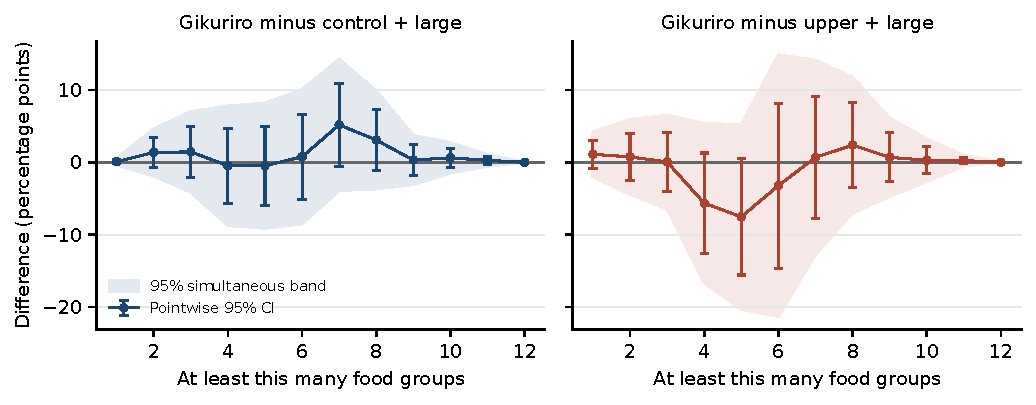
\includegraphics[width=\textwidth]{../output/figures/diet_thresholds.pdf}
\caption{Diet-threshold contrasts at the same expected budget}\label{fig:thresholds}
\begin{minipage}{\textwidth}\footnotesize
\emph{Notes:} Differences are Gikuriro minus the indicated cash policy, in percentage points. Thin intervals are pointwise 95 percent confidence intervals. Shading is a 95 percent simultaneous band over all \FamilyN\ primary comparisons. Estimates use the same village-clustered ANCOVA design as Table \ref{tab:itt}. These are threshold effects, not an estimated joint distribution of household-level treatment effects.
\end{minipage}
\end{figure}

Figure \ref{fig:frontier} places the mean results in a broader budget comparison. The cash envelope is the highest fitted mean attainable by a lottery over observed cash packages and control at each expected budget. At the Gikuriro budget its selected segment combines lower and large cash. Gikuriro's ANCOVA contrast is \LowerLargeDietEstimate\ groups, with interval [\LowerLargeDietSimLo, \LowerLargeDietSimHi]. Universal upper cash is feasible and lies above Gikuriro in fitted mean, but it is not the fitted optimum. Policy selection requires the joint comparisons reported next.

\begin{figure}[t]
\centering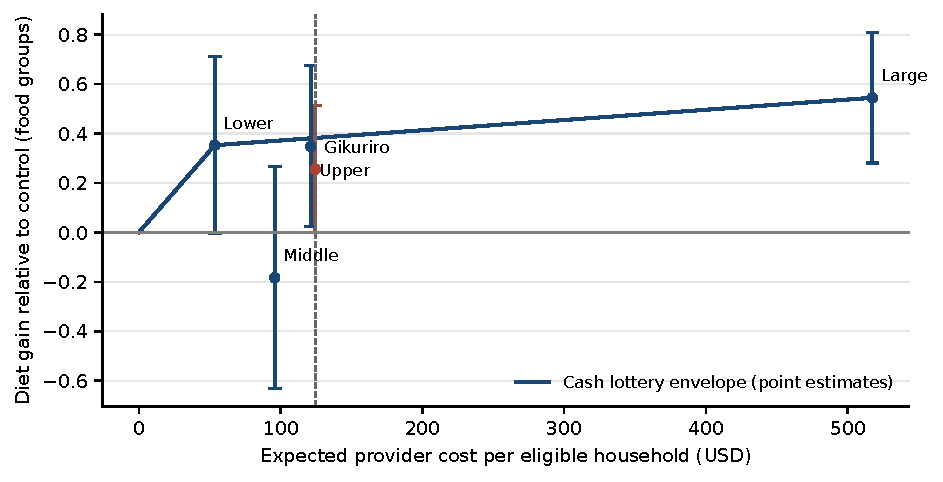
\includegraphics[width=.95\textwidth]{../output/figures/budget_frontier.pdf}
\caption{The diet-budget frontier over observed cash packages}\label{fig:frontier}
\begin{minipage}{\textwidth}\footnotesize
\emph{Notes:} Points are package ITTs on HDDS; intervals are pointwise 95 percent confidence intervals. The line is the fitted cash-only envelope, allowing resources to remain unspent. Straight segments describe randomized coverage or package mixtures, not a continuous household response to transfer amount. The vertical line marks the Gikuriro cost. Cost inputs are held fixed; uncertainty in those inputs is not included in the intervals.
\end{minipage}
\end{figure}

\subsection{Economic outcomes and possible mechanisms}

Table \ref{tab:secondary} documents changes in other household outcomes. Large cash increases the source productive-asset IHS measure by \LargeAssetsEstimate\ units, with standard error \LargeAssetsSE. This effect survives the secondary-family Holm correction. Gikuriro increases the saving-stock IHS measure by \GikuriroSavingEstimate\ units, with standard error \GikuriroSavingSE. Its unadjusted $p$-value is \GikuriroSavingP; the Holm value is \GikuriroSavingHolmP, which places the result close to, but above, the conventional 5 percent family threshold. The result is therefore suggestive at that threshold rather than decisive under the wider secondary family.

The saving and productive-asset patterns help interpret the diet evidence. Resources can be carried forward through a saving group or invested in productive assets. A diet measured on one day does not record all of those uses. Equation \eqref{eq:household} provides one reason why a saving opportunity can improve intertemporal allocation while leaving a current dietary index unchanged. The trial bundles agricultural inputs, nutrition advice, and saving activities, so this interpretation remains a mechanism consistent with the evidence, not an estimated causal pathway.

\begin{table}[p]
\centering\caption{Secondary household outcomes}\label{tab:secondary}
\resizebox{\textwidth}{!}{\begin{tabular}{lrrrrr}
\toprule
 & Gikuriro & Lower & Middle & Upper & Large \\
\midrule
Consumption (IHS) & $-0.093$ & $0.118$ & $-0.001$ & $0.083$ & $0.327$ \\
 & (0.099) & (0.116) & (0.128) & (0.120) & (0.108) \\
 & [1.000] & [1.000] & [1.000] & [1.000] & [0.245] \\
Productive assets (IHS) & $0.008$ & $0.271$ & $0.248$ & $0.246$ & $0.780^{***}$ \\
 & (0.103) & (0.127) & (0.175) & (0.135) & (0.118) \\
 & [1.000] & [1.000] & [1.000] & [1.000] & [$<0.001$] \\
Saving stock (IHS) & $1.186^{*}$ & $-0.009$ & $-0.286$ & $0.353$ & $0.720$ \\
 & (0.338) & (0.447) & (0.539) & (0.525) & (0.322) \\
 & [0.052] & [1.000] & [1.000] & [1.000] & [1.000] \\
Borrowing stock (IHS) & $0.056$ & $-0.667$ & $-0.714$ & $-0.830$ & $-0.325$ \\
 & (0.358) & (0.339) & (0.434) & (0.375) & (0.388) \\
 & [1.000] & [1.000] & [1.000] & [1.000] & [1.000] \\
Health knowledge index & $-0.062$ & $0.273$ & $0.041$ & $0.068$ & $0.039$ \\
 & (0.366) & (0.488) & (0.410) & (0.373) & (0.474) \\
 & [1.000] & [1.000] & [1.000] & [1.000] & [1.000] \\
Sanitation practices index & $-0.207$ & $0.337$ & $-0.229$ & $0.323$ & $0.112$ \\
 & (0.227) & (0.363) & (0.286) & (0.283) & (0.298) \\
 & [1.000] & [1.000] & [1.000] & [1.000] & [1.000] \\
Purchased food (IHS) & $-0.172$ & $0.058$ & $0.024$ & $0.264$ & $0.267$ \\
 & (0.177) & (0.192) & (0.187) & (0.188) & (0.170) \\
 & [1.000] & [1.000] & [1.000] & [1.000] & [1.000] \\
Own-produced food (IHS) & $0.125$ & $0.556$ & $-0.601$ & $-0.558$ & $0.968$ \\
 & (0.322) & (0.378) & (0.427) & (0.556) & (0.393) \\
 & [1.000] & [1.000] & [1.000] & [1.000] & [1.000] \\
Households (range across outcomes) & 1751 & 1751 & 1751 & 1751 & 1751 \\
Villages (range across outcomes) & 248 & 248 & 248 & 248 & 248 \\
\bottomrule
\end{tabular}
}
\begin{minipage}{\textwidth}\footnotesize
\emph{Notes:} Weighted ANCOVA assignment effects relative to control. Standard errors are in parentheses. Brackets and stars use Holm adjustment over 96 distinct secondary outcome/arm and outcome/policy comparisons; eight duplicated Gikuriro/control entries do not add tests. IHS coefficients are changes in the source transformation, not percentage changes. Purchased and own-produced food use weekly-recall source values, including zeros; no price-base conversion is asserted. Knowledge and sanitation use the source indices.
\end{minipage}
\end{table}

The food-category results provide a more direct view of dietary composition. Large cash increases reported cereal and oil consumption, with Holm-adjusted evidence after the 80 food-category/arm comparisons. Other categories have intervals compatible with a range of changes. These household responses do not identify child nutrient intake. Heterogeneity tests using baseline diet and baseline consumption splits also fail to establish systematic differences: the smallest Holm-adjusted $p$-value is \HetMinP. This limits claims that the existing trial reveals a reliable rule for targeting Gikuriro to households with the poorest initial diets.

\section{Population distributions and policy choice}

\subsection{Selection-aware diet comparisons}

Equation \eqref{eq:hajek} constructs coherent arm distributions using known assignment probabilities. Among identified diets, Gikuriro's mean contrast is \HajekControlLargeEstimate\ groups against control/large cash and \HajekLowerLargeEstimate\ against lower/large cash. The respective simultaneous intervals are [\HajekControlLargeSimLo, \HajekControlLargeSimHi] and [\HajekLowerLargeSimLo, \HajekLowerLargeSimHi]. These observed-outcome estimates differ from the pooled ANCOVA results because they change both adjustment and block representation. Neither is an unrestricted baseline-population effect in the presence of selection.

Table \ref{tab:populationbounds} retains every baseline eligible household and uses the interval information in its food responses. For mean diversity, all reported identification regions cross zero. For the six-group shortfall, the sample regions against lower/large and upper/large cash favor cash, but their simultaneous uncertainty bands cross zero. The sample sign therefore supplies no significant population ranking. Missing-outcome assignments cannot be dismissed merely because the complete-case sample is large.

\begin{table}[t]
\centering\caption{Population-aligned identification regions and sampling bands}\label{tab:populationbounds}
\resizebox{\textwidth}{!}{\begin{tabular}{lrrrrrr}
\toprule
Outcome & Cash policy & Observed & Bound lo. & Bound hi. & 95\% lo. & 95\% hi. \\
\midrule
HDDS & Control + Large & 0.039 & -0.275 & 0.323 & -0.793 & 0.856 \\
HDDS & Lower + Large & -0.237 & -0.574 & 0.101 & -1.215 & 0.804 \\
HDDS & Upper + Large & -0.147 & -0.293 & 0.005 & -0.987 & 0.719 \\
Shortfall ($z=6$) & Control + Large & -0.003 & -0.029 & 0.020 & -0.089 & 0.081 \\
Shortfall ($z=6$) & Lower + Large & -0.039 & -0.063 & -0.007 & -0.131 & 0.070 \\
Shortfall ($z=6$) & Upper + Large & -0.030 & -0.050 & -0.025 & -0.136 & 0.062 \\
\bottomrule
\end{tabular}
}
\begin{minipage}{\textwidth}\footnotesize
\emph{Notes:} Positive contrasts favor Gikuriro. ``Observed'' uses identified diets and inverse block-assignment weights. Bound endpoints use all baseline eligibles and item-informed score intervals. The last two columns cover the lower and upper endpoints using the \BoundFamilyN-test simultaneous endpoint family across all policy pairs and objectives. They are a cluster-asymptotic confidence envelope for the identification region, not a narrower confidence interval obtained by treating missing diets as observed. Costs and transport assumptions remain conditional.
\end{minipage}
\end{table}

Figure \ref{fig:coherent} gives the corresponding survival comparisons. Its point estimates derive from a single positive-weight distribution in each arm; their means and shortfalls obey the discrete distribution identities exactly. The shaded population envelopes allow both sampling uncertainty and all diets consistent with observed food responses. Across all twelve survival thresholds and all twelve linear shortfalls, the data do not establish either increasing or increasing-concave dominance of Gikuriro over its fitted best cash benchmark. Oils, sweets and condiments count in HDDS, so even a dominance result would concern measured household food access rather than child nutritional adequacy.

\begin{figure}[t]
\centering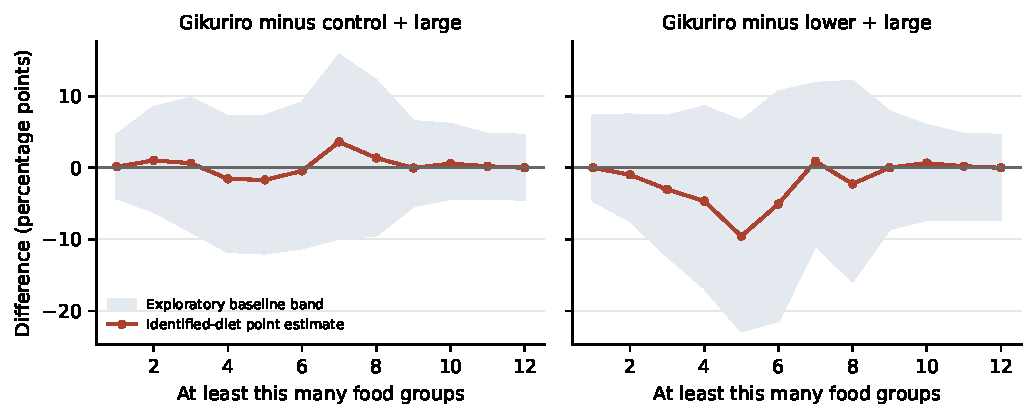
\includegraphics[width=\textwidth]{../output/figures/coherent_thresholds.pdf}
\caption{Coherent dietary distributions allowing incomplete outcomes}\label{fig:coherent}
\begin{minipage}{\textwidth}\footnotesize
\emph{Notes:} Point estimates compare identified-diet H\'ajek distributions. Shading covers baseline-population contrast endpoints simultaneously over the declared \BoundFamilyN-test family. The complete-case point estimate need not lie in every realized identification region, because observation normalization changes the denominator. No household nutrient or sharp-null randomization claim is implied.
\end{minipage}
\end{figure}

\subsection{Which allocations can the evidence defend?}

Lower/large cash has the highest fitted mean under both estimators. Under the coherent distribution, choosing Gikuriro instead has fitted regret \GKFittedRegret\ groups. Table \ref{tab:regret} and Figure \ref{fig:regret} separate this fitted loss from its uncertainty. All nine policies remain in the mean-optimality confidence set. The observed-diet upper regret bounds are \GKObservedRegretUpper\ for Gikuriro and \LowerLargeObservedRegretUpper\ for lower/large cash. Permitting arbitrary missing diets raises the baseline-population upper bounds to \GKPopulationRegretUpper\ and \LowerLargePopulationRegretUpper, respectively.

An organization requiring a quarter-group or half-group regret guarantee cannot certify any candidate from these bands. A one-group tolerance admits lower/large cash and pure lower cash in the population-bound exercise. That is a loose guarantee on a twelve-group proxy, not proof that either is the optimum or socially preferred. It remains conditional on the cluster approximation, fixed provider costs and stable delivery. In the observed-diet six-group-shortfall exercise, control and middle cash are excluded from the optimality set; permitting missing diets returns all nine candidates to the conservative set. Objectives and selection assumptions thus change what can be ruled out even while leaving the fitted winner unchanged.

\begin{table}[t]
\centering\caption{Mean-diet policy regret: point estimates and upper bounds}\label{tab:regret}
\resizebox{\textwidth}{!}{\begin{tabular}{lrrrr}
\toprule
Policy & Fitted HDDS & Fitted regret & Observed 95\% upper & Population 95\% upper \\
\midrule
Gikuriro & 5.029 & 0.237 & 0.878 & 1.283 \\
Control & 4.875 & 0.392 & 1.010 & 1.429 \\
Lower & 5.250 & 0.016 & 0.684 & 0.997 \\
Middle & 4.503 & 0.763 & 1.725 & 2.104 \\
Upper & 5.175 & 0.092 & 0.835 & 1.109 \\
Control + Large & 4.991 & 0.276 & 0.861 & 1.269 \\
Lower + Large & 5.267 & 0.000 & 0.616 & 0.898 \\
Middle + Large & 4.561 & 0.705 & 1.621 & 2.000 \\
Upper + Large & 5.176 & 0.091 & 0.831 & 1.105 \\
\bottomrule
\end{tabular}
}
\begin{minipage}{\textwidth}\footnotesize
\emph{Notes:} Regret is relative to the best of these nine candidates, in HDDS groups. Observed-outcome bounds use all \PairFamilyN\ distinct pairwise tests; population bounds use all \BoundFamilyN\ distinct contrast endpoints. Costs are fixed. Zero fitted regret is selection of a sample winner, while every policy's mean-regret lower confidence bound is zero. The bounds do not identify latent dietary preferences or compare all imaginable interventions.
\end{minipage}
\end{table}

\begin{figure}[t]
\centering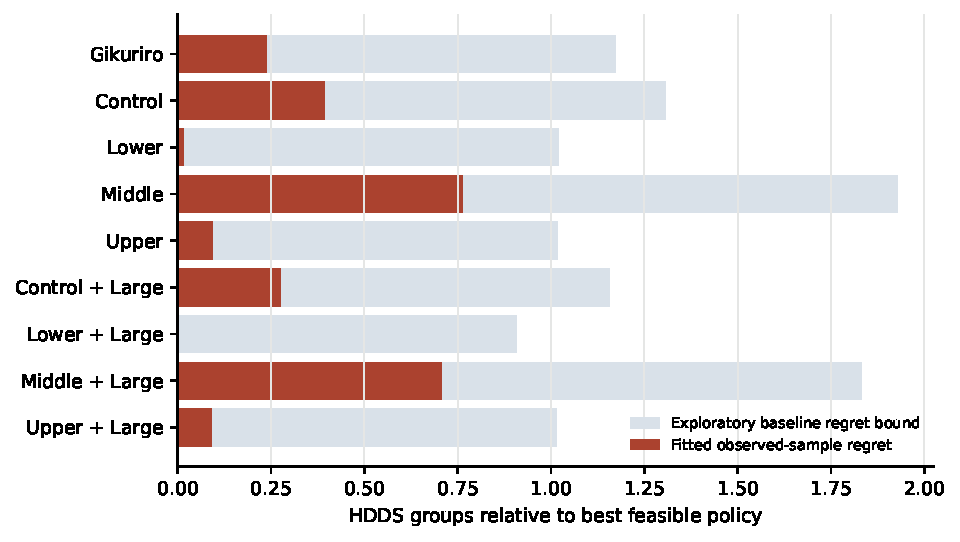
\includegraphics[width=.95\textwidth]{../output/figures/policy_regret.pdf}
\caption{A fitted winner and the uncertainty in its opportunity cost}\label{fig:regret}
\end{figure}

\section{Robustness, missing data, and policy accounting}

\subsection{Weighting and measurement}

Appendix Table \ref{tab:robustness} compares the mean-diet policy contrasts using block controls without a baseline outcome, equal household weights, equal village weights, the supplied diet score, and only households with observed baseline diets. The Gikuriro/control-large estimate remains positive across these specifications. The upper/large contrast is negative under survey weighting and positive under equal household or village weighting. This sign sensitivity is economically relevant: the survey-weighted estimand gives more representation to households in the original target population, while the alternatives change the composition of that population.

Using the supplied score instead of the reconstructed score changes some estimates modestly. The measurement decision matters most for the interpretation of threshold outcomes: a replacement value of 4.463 cannot be understood as an observed integer number of food groups. The primary specification consequently preserves missingness and exposes it to the attrition analysis. The sensitivity using the supplied score allows a reader to assess whether that choice drives the substantive conclusion.

\subsection{Attrition and incomplete food modules}

High overall retention does not by itself establish the absence of selection. Table \ref{tab:design} reports the observed diet sample and baseline-weighted retention in each arm. In the missing-outcome analysis, a household can be absent from endline or present with an incomplete food module. Both count as unobserved for primary diet analysis. Appendix Table \ref{tab:retention} estimates observation effects on the full baseline eligible population. Upper cash increases the probability of an observed diet by \UpperRetention\ percentage points, with standard error \UpperRetentionSE\ and a five-test Holm $p$-value of \UpperRetentionHolmP. The complete-case comparison involving upper cash therefore needs particular caution. Random assignment alone does not remove this selection problem.

For a bounded outcome $v\in[\underline v,\overline v]$, let $r_a$ be the baseline-weighted observation share in arm $a$ and $\bar v_{a,obs}$ the weighted observed mean. The full arm mean lies in
\begin{equation}
 [r_a\bar v_{a,obs}+(1-r_a)\underline v,\;
   r_a\bar v_{a,obs}+(1-r_a)\overline v]. \label{eq:bounds}
\end{equation}
This formula describes the coarse all-or-nothing case. The item-informed intervals and assignment probabilities in Table \ref{tab:populationbounds} use more information and include endpoint sampling uncertainty. Appendix Table \ref{tab:bounds} preserves the initial coarse sample bounds as an audit crosswalk; those older bounds are neither block aligned nor confidence intervals. The replication also varies every unidentified score between its lower and upper endpoint along a common fraction from zero to one. That missing-mean scenario is transparent, but it does not restrict the full worst-case region or establish that missing households share a common food response.

\subsection{Crosswalk and finite-cluster diagnostics}

Appendix Table \ref{tab:crosswalk} reconstructs the original household diet specification using the corrected archive, pooled smaller cash arms and the original fixed, source-selected control list. Gikuriro and large-cash effects reproduce the original paper's published rounding. Splitting the smaller arms, removing the selected controls, replacing supplied outcomes by integer scores, and replacing supplied baseline controls by observed integer baselines explain the path to the current ANCOVA estimates. No new LASSO selection is performed, and the corrected release's one-household difference remains disclosed.

CR2 and Satterthwaite inference leave the mean policy ranking unresolved (Appendix Table \ref{tab:cr2}). The effective degrees of freedom are contrast specific and substantially below the total village count for small cash arms. Weight and score concentration are also uneven: the number of observed villages overstates the information in some contrasts. Tables \ref{tab:weightsupport} and \ref{tab:leaveout} report concentration and omission diagnostics. The lower/large contrast stays negative when any one village or block is omitted; its interval still includes zero. Sign stability is therefore distinct from statistical precision.

\subsection{Child outcomes and households outside eligibility}

The corrected individual panel contains standardized scores for height, weight and upper arm circumference. I estimate a separate exploratory fifteen-test assignment family among baseline-eligible households' endline children classified as due for anthropometry. These source-defined samples and inherited score cleaning differ from the integer diet reconstruction. The ANCOVA uses the supplied baseline score with a missing indicator and block controls. It does not repeat the original study's larger source-selected anthropometric control list, nor correct attrition by an invented propensity model. None of these estimates survives the declared Holm family (Appendix Table \ref{tab:populations}). This does not reverse the original paper's child-growth evidence under its own prespecified specifications.

For baseline-ineligible households I estimate diet, consumption and saving assignment effects, with a separate fifteen-test Holm family. No result survives that correction. This is evidence about the measured ineligible sample under original village assignments. Selection and imprecision remain, so it is not an identified zero spillover or a measure of all public-service benefits. Neither extension establishes a Catholic-specific channel: religious affiliation was not randomized.

\subsection{Magnitude and omitted benefits}

The simplest calibration is the reach of the large package. At the original accounting costs, replacing universal Gikuriro with large cash/control changes the share of villages receiving a package from one to approximately one quarter. In a hypothetical population of otherwise comparable villages, the expected diet gain from that policy is the large-cash ITT multiplied by its coverage probability. This multiplication follows directly from the policy definition; it does not require an assumption that food spending or household welfare responds linearly to dollars.

For the upper/large mixture, equation \eqref{eq:breakeven} gives a fitted omitted-benefit requirement of \UpperLargeBreakEven\ diet-equivalent groups per eligible household for Gikuriro to match the cash policy. This number is the negative of the estimated diet contrast when that contrast favors cash. The simultaneous interval for the underlying contrast runs from \UpperLargeDietSimLo\ to \UpperLargeDietSimHi, so even the sign of the omitted-benefit requirement is unresolved. A researcher cannot conclude that unmeasured benefits of that magnitude exist. Conversely, the data do not justify setting all future or public-service consequences to zero.

Cost uncertainty creates a further limitation. The large-cash/control coverage probability changes proportionally with the assumed Gikuriro budget and inversely with large-cash cost. The upper/large mixture places a particularly small fraction in the large package because upper cash nearly exhausts the budget already. Errors in overhead allocation or compliance accounting can therefore change the relevant cash mix. Program redesign, inflation, or a different implementation scale would require new cost evidence; the reported numbers describe the original experiment.

The replication rebuilds the complete feasible policy set on a five-by-five relative-cost grid, varying Gikuriro and cash costs by factors 0.75, 0.90, 1, 1.10 and 1.25. It also uses the actual accounting decomposition $c_a^{elig}=c_a^{benef}[1-s_a+s_a r_a]$, where $s_a$ is the avertable share and $r_a$ compliance, to vary common take-up and Gikuriro's avertable share. Outcome effects are held fixed in these accounting scenarios; a change in take-up could change effects as well, so these are not forecasts. The generated \texttt{cost\_scenarios.csv} records every rebuilt vertex and its fitted value. All pairs are enumerated regardless of cost ordering, a property verified against linear-program solutions.

The upper package is near the feasibility boundary: its original cost is only \$\ProviderSavingUpper\ below the budget. A small relative-cost change can remove it as a pure feasible policy. Fixed activation costs create a different problem. A cost of $F_a\ind\{n_a>0\}+m_a n_a$ cannot generally be represented by the constant per-household constraint in equation \eqref{eq:planner}. The present grid conditions on an allocated unit-cost convention; solving a hard finite-budget problem with genuine activation costs would require eligible counts, capacity and fixed-cost accounts at the proposed scale. I do not manufacture those inputs.

Lower/large cash remains the fitted mean optimum in every reported cost scenario. This stability holds effects fixed at the initial ANCOVA estimates; it does not resolve their sampling uncertainty or establish that changing participation leaves outcomes unchanged.

\section{Discussion}

The estimates leave a choice among imperfectly ranked allocations. The mean/control-large comparison restates the original cost-effectiveness question. The added evidence concerns coherent food-access distributions, incomplete responses and policy regret. Lower/large cash is the fitted optimum, but its population regret cannot be certified below a half group by the reported bands. An organization requiring that precision needs additional evidence rather than a preferred wording of the existing mean comparison.

The analysis also changes how a fixed-cost benchmark can be read. A line between two package outcomes describes an implementable lottery over those packages. It says nothing about the outcome of giving every household a transfer equal to the weighted average of the two amounts. For a mean objective, the two descriptions may be used interchangeably only under an additional response restriction. For a shortfall-sensitive objective, agreement of mean responses would still not establish agreement of distributions. Researchers and implementing organizations should state which intervention is represented by an interpolation.

Several features prevent a broader welfare conclusion. HDDS is a household proxy and does not tell me how food is allocated to the child whom Gikuriro targets. The cash and in-kind interventions were not delivered on identical schedules: the original study reports earlier cash receipt and slower rollout of Gikuriro. The observation window may consequently favor immediate cash effects relative to activities whose returns take time. The control group subsequently received treatment, limiting identification of sustained differences. Ineligible residents may benefit from services, and cross-village prices or saving networks can respond to coverage. I do not measure total public-service benefits or claim an absence of these spillovers.

The model suggests useful evidence for a further evaluation. Repeated diet and expenditure observations would distinguish persistent improvements from survey-day variation. Measurements of saving-group terms, fees, returns, and withdrawals would make the intertemporal mechanism testable. A design that randomizes both package intensity and the share of villages served would directly estimate the scale margin on which the lottery comparison currently relies. Child-level nutrient measures would connect household food access to the nutritional target more closely. These extensions require new data; they cannot be supplied by additional transformations of the existing panel.

For the current decision, the practical implication is to separate delivery reach, current food access, and longer-term household resources. If an organization values universal contact or a minimum package in every village, control/large cash is not a feasible substitute even though it respects expected cost. If it is prepared to allocate assistance by lottery, the experiment supplies the outcomes needed for the conditional comparison. The distinction should be part of the decision rather than hidden in a cost-effectiveness ratio.

\section{Conclusion}

I use the randomized evaluation of CRS' Gikuriro program to compare observed aid packages at the same expected budget. Lower/large cash has the highest fitted mean, while all nine candidates remain statistically compatible with mean optimality. Selection-aware distributions and simultaneous regret bounds show how much decision uncertainty remains. A loose one-group guarantee is attainable for that fitted cash policy under the stated approximation; a half-group guarantee is not. These findings extend the parent study's cost-effectiveness analysis without identifying a new experiment, a Catholic-specific mechanism, or a general superiority of cash.

The theoretical framework explains why current dietary evidence need not track the full value of an intervention that changes saving opportunities. The trial informs aid reach and current diet; ranking social welfare requires evidence on future returns, child nutrition, spillovers, and costs at scale.

\clearpage
\begin{singlespace}\small
\begin{thebibliography}{99}
\bibitem[Banerjee and Duflo(2007)]{banerjeeduflo2007} Banerjee, Abhijit V., and Esther Duflo. 2007. ``The Economic Lives of the Poor.'' \emph{Journal of Economic Perspectives} 21(1): 141--167. \href{https://doi.org/10.1257/jep.21.1.141}{doi:10.1257/jep.21.1.141}.
\bibitem[Currie and Gahvari(2008)]{curriegahvari2008} Currie, Janet, and Firouz Gahvari. 2008. ``Transfers in Cash and In-Kind: Theory Meets the Data.'' \emph{Journal of Economic Literature} 46(2): 333--383. \href{https://doi.org/10.1257/jel.46.2.333}{doi:10.1257/jel.46.2.333}.
\bibitem[Cunha et al.(2019)]{cunha2019} Cunha, Jesse M., Giacomo De Giorgi, and Seema Jayachandran. 2019. ``The Price Effects of Cash Versus In-Kind Transfers.'' \emph{Review of Economic Studies} 86(1): 240--281. \href{https://doi.org/10.1093/restud/rdy018}{doi:10.1093/restud/rdy018}.
\bibitem[Egger et al.(2022)]{egger2022} Egger, Dennis, Johannes Haushofer, Edward Miguel, Paul Niehaus, and Michael Walker. 2022. ``General Equilibrium Effects of Cash Transfers: Experimental Evidence from Kenya.'' \emph{Econometrica} 90(6): 2603--2643. \href{https://doi.org/10.3982/ECTA17945}{doi:10.3982/ECTA17945}.
\bibitem[FAO(2011)]{fao2011} Food and Agriculture Organization of the United Nations. 2011. \emph{Guidelines for Measuring Household and Individual Dietary Diversity}. Gina Kennedy, Terri Ballard, and Marie-Claude Dop. Rome: FAO. \url{https://www.fao.org/fileadmin/user_upload/wa_workshop/docs/FAO-guidelines-dietary-diversity2011.pdf}.
\bibitem[Foster et al.(1984)]{foster1984} Foster, James, Joel Greer, and Erik Thorbecke. 1984. ``A Class of Decomposable Poverty Measures.'' \emph{Econometrica} 52(3): 761--766. \href{https://doi.org/10.2307/1913475}{doi:10.2307/1913475}.
\bibitem[Haushofer and Shapiro(2016)]{haushofer2016} Haushofer, Johannes, and Jeremy Shapiro. 2016. ``The Short-Term Impact of Unconditional Cash Transfers to the Poor: Experimental Evidence from Kenya.'' \emph{Quarterly Journal of Economics} 131(4): 1973--2042. \href{https://doi.org/10.1093/qje/qjw025}{doi:10.1093/qje/qjw025}.
\bibitem[Imbens and Koles\'ar(2016)]{imbenskolesar2016} Imbens, Guido W., and Michal Koles\'ar. 2016. ``Robust Standard Errors in Small Samples: Some Practical Advice.'' \emph{Review of Economics and Statistics} 98(4): 701--712. \href{https://doi.org/10.1162/REST_a_00552}{doi:10.1162/REST\_a\_00552}.
\bibitem[Kitagawa and Tetenov(2018)]{kitagawa2018} Kitagawa, Toru, and Aleksey Tetenov. 2018. ``Who Should Be Treated? Empirical Welfare Maximization Methods for Treatment Choice.'' \emph{Econometrica} 86(2): 591--616. \href{https://doi.org/10.3982/ECTA13288}{doi:10.3982/ECTA13288}.
\bibitem[Manski(2004)]{manski2004} Manski, Charles F. 2004. ``Statistical Treatment Rules for Heterogeneous Populations.'' \emph{Econometrica} 72(4): 1221--1246. \href{https://doi.org/10.1111/j.1468-0262.2004.00530.x}{doi:10.1111/j.1468-0262.2004.00530.x}.
\bibitem[McIntosh(2025)]{data2025} McIntosh, Craig. 2025. ``Replication Package EJ MS 20220682.'' Corrected dataset, created July 15, 2025, nominal publication date May 23, 2024, version 1. Zenodo. \href{https://doi.org/10.5281/zenodo.15881329}{doi:10.5281/zenodo.15881329}. Accessed September 30, 2026. CC BY 4.0. The record lists McIntosh as creator; the underlying paper is coauthored with Andrew Zeitlin.
\bibitem[McIntosh and Zeitlin(2024)]{mcintosh2024} McIntosh, Craig, and Andrew Zeitlin. 2024. ``Cash Versus Kind: Benchmarking a Child Nutrition Program Against Unconditional Cash Transfers in Rwanda.'' \emph{Economic Journal} 134(664): 3360--3389. \href{https://doi.org/10.1093/ej/ueae050}{doi:10.1093/ej/ueae050}.
\end{thebibliography}
\end{singlespace}\normalsize

\clearpage\appendix
\section{Theory proofs and scope}

\begin{proof}[Proof of Proposition 1]
Substitute $s=w+t-f$ into equation \eqref{eq:household}. The first-order condition is
\[
 \frac1{f-\underline f}=\frac{\beta R}{R(w+t-f)+y}.
\]
Strict concavity gives the unique interior optimum in the proposition.
Differentiation gives $\partial f^*/\partial t=1/(1+\beta)$,
$\partial s^*/\partial t=\beta/(1+\beta)$,
$\partial f^*/\partial R=-y/[(1+\beta)R^2]$, and
$\partial s^*/\partial R=y/[(1+\beta)R^2]$.
The envelope theorem gives $\partial U^*/\partial R=\beta s^*/(Rs^*+y)>0$
when $s^*>0$. The interior condition is
$\beta(w+t-\underline f)>y/R$. If it fails, the nonnegativity constraint
binds and $s^*=0$. Equation \eqref{eq:diet} is monotone and locally constant
between thresholds, establishing the diversity claims and the first corollary.
\end{proof}

\begin{proof}[Proof of Proposition 2]
Conditional independence of the policy lottery and potential outcomes gives
$\Pr(D_q\leq d)=\sum_a q_a\Pr(D(a)\leq d)$ by iterated expectation.
The same argument applies to any integrable objective $v$. The feasible set
in equation \eqref{eq:planner} is a nonempty compact polytope, so a linear
objective has a maximizing extreme point. An extreme point with a slack cost
constraint has at most one positive component: otherwise a small shift between
two components preserves the probability sum and feasibility. With binding
cost, any three positive components admit a nonzero perturbation solving both
$\sum_a h_a=0$ and $\sum_a c_a h_a=0$. Small positive and negative multiples
are feasible, contradicting extremality. At most two components are therefore
positive. Solving the two binding equalities gives equation \eqref{eq:mix}.
Setting the cheaper package to control proves the coverage corollary.
\end{proof}

\begin{proof}[Proof of Proposition 3]
On the simultaneous coverage event every term $\mu_b-\mu_a$ lies between its pairwise bounds. Taking maxima preserves both inequalities and gives the regret bounds. For any optimal $a$, every $\mu_b-\mu_a\leq0$, so $L_{ba}\leq0$ for every $b$. The policy is consequently in the stated set. If the largest upper bound is no greater than $\epsilon$, the regret inequality proves the tolerance claim. Using a confidence upper bound for every interval-outcome upper endpoint repeats the argument uniformly over admissible missing diets.
\end{proof}

For a bounded integer score, an increasing function can be written as
$v(d)=v(0)+\sum_{k=1}^{12}[v(k)-v(k-1)]\ind\{d\geq k\}$.
All coefficients are nonnegative. Thus weakly higher survival probabilities
imply weakly higher expected increasing objectives. Concavity places the
corresponding restrictions on increments, and negative lower partial moments
give the usual increasing-concave ordering. Separate finite-sample ANCOVA
threshold estimates need not form an exactly monotone fitted distribution;
the assignment-weighted distributions in the revision form one coherent CDF
per arm, and the code verifies both discrete identities. There is no established
dominance of Gikuriro over the fitted best cash policy under the simultaneous
population bands.

\clearpage
\section{Additional empirical exhibits}

\begin{table}[htbp]
\centering\caption{Food-module information in the baseline eligible cohort}\label{tab:intervalcounts}
\begin{tabular}{lrrrr}
\toprule
Arm & Baseline & Identified & Partial & Unobserved \\
\midrule
Control & 521 & 498 & 6 & 17 \\
Gikuriro & 540 & 522 & 2 & 16 \\
Lower & 165 & 160 & 0 & 5 \\
Middle & 154 & 149 & 0 & 5 \\
Upper & 167 & 164 & 3 & 0 \\
Large & 246 & 237 & 4 & 5 \\
\bottomrule
\end{tabular}

\begin{minipage}{\textwidth}\footnotesize
\emph{Notes:} Identified includes complete modules and partial modules that nevertheless identify all twelve groups. Partial denotes an interval of width between one and eleven. Unobserved denotes width twelve, including absent endline households. Every baseline eligible household occurs once. These counts are not a missing-at-random adjustment.
\end{minipage}
\end{table}

\begin{table}[htbp]
\centering\caption{Crosswalk from the original diet specification}\label{tab:crosswalk}
\resizebox{\textwidth}{!}{\begin{tabular}{lrrrrr}
\toprule
Specification & GK & GK SE & Large & Large SE & N \\
\midrule
Original controls, pooled cash & 0.192 & 0.122 & 0.550 & 0.126 & 1751 \\
Original controls, split cash & 0.201 & 0.123 & 0.558 & 0.126 & 1751 \\
Supplied-score lag only & 0.235 & 0.131 & 0.530 & 0.131 & 1751 \\
Integer outcome, supplied lag & 0.258 & 0.130 & 0.547 & 0.133 & 1728 \\
Integer outcome and baseline & 0.255 & 0.131 & 0.545 & 0.134 & 1728 \\
\bottomrule
\end{tabular}
}
\begin{minipage}{\textwidth}\footnotesize
\emph{Notes:} Original controls reproduce the fixed covariate list in the corrected deposit's \texttt{CovariateLists.xlsx} and \texttt{Table\_3.do}, including the supplied lag. Pooled means the three smaller cash arms share a coefficient. Split estimates them separately. Collinear supplied baseline columns are omitted in the stated order, matching the identified regression span. Later rows change the control list and integer-score missingness sequentially. Standard errors use village CR1. The final row is this project's original ANCOVA. Published rounding, rather than an exact recovery of a withdrawn dataset, is the comparison.
\end{minipage}
\end{table}

\begin{table}[htbp]
\centering\caption{Mean-diet small-cluster sensitivity}\label{tab:cr2}
\resizebox{\textwidth}{!}{\begin{tabular}{lrrrrr}
\toprule
Contrast & Effect & CR2 SE & Satt. df & Pointwise $p$ & Effective clusters \\
\midrule
Gikuriro & 0.255 & 0.139 & 91.8 & 0.069 & 28.0 \\
Lower & 0.353 & 0.196 & 28.8 & 0.083 & 10.1 \\
Middle & -0.183 & 0.256 & 21.2 & 0.482 & 3.9 \\
Upper & 0.348 & 0.180 & 26.2 & 0.065 & 10.5 \\
Large & 0.545 & 0.142 & 47.9 & $<0.001$ & 34.4 \\
GK vs. Control + Large & 0.124 & 0.126 & 96.7 & 0.327 & 27.8 \\
GK vs. Lower + Large & -0.127 & 0.175 & 34.6 & 0.474 & 12.9 \\
\bottomrule
\end{tabular}
}
\begin{minipage}{\textwidth}\footnotesize
\emph{Notes:} Same WLS coefficient specification as the main ANCOVA; CR2 changes its variance estimate. Satterthwaite degrees of freedom use the independent, homoskedastic whitened-error working model. Effective clusters are the inverse concentration of squared cluster scores for the indicated contrast. These are pointwise diagnostic $p$-values, not the primary simultaneous policy family or exact randomization tests. Working-model sandwich expectation identities are verified in code.
\end{minipage}
\end{table}

\begin{table}[htbp]
\centering\caption{Village weight support among complete diets}\label{tab:weightsupport}
\resizebox{\textwidth}{!}{\begin{tabular}{lrrr}
\toprule
Arm & Villages & Effective weight villages & Maximum village weight (\%) \\
\midrule
Control & 74 & 44.6 & 5.4 \\
Gikuriro & 74 & 51.7 & 5.6 \\
Lower & 22 & 16.7 & 10.7 \\
Middle & 22 & 12.6 & 17.9 \\
Upper & 22 & 15.0 & 15.1 \\
Large & 34 & 24.1 & 8.9 \\
\bottomrule
\end{tabular}
}
\begin{minipage}{\textwidth}\footnotesize
\emph{Notes:} Village weights sum source sampling weights over observed eligible diets. Effective support is $(\sum_j W_j)^2/\sum_j W_j^2$. It concerns weight concentration, not the contrast-specific score concentration in Table \ref{tab:cr2}.
\end{minipage}
\end{table}

\begin{table}[htbp]
\centering\caption{Omitting each village and each randomization block}\label{tab:leaveout}
\begin{tabular}{lrrrr}
\toprule
Omitted unit & Cash comparator & Minimum effect & Maximum effect & Fits \\
\midrule
Village & Control + Large & 0.087 & 0.172 & 248 \\
Village & Lower + Large & -0.209 & -0.058 & 248 \\
Village & Upper + Large & -0.143 & 0.019 & 248 \\
Block & Control + Large & 0.068 & 0.171 & 22 \\
Block & Lower + Large & -0.219 & -0.038 & 22 \\
Block & Upper + Large & -0.137 & -0.006 & 22 \\
\bottomrule
\end{tabular}

\begin{minipage}{\textwidth}\footnotesize
\emph{Notes:} Minimum and maximum reestimated Gikuriro-minus-policy mean coefficients. Each fit recomputes baseline imputation, block indicators and covariance on the remaining data, holding original package costs fixed. Omission ranges are sensitivity diagnostics, not confidence intervals.
\end{minipage}
\end{table}

\begin{table}[htbp]
\centering\caption{Available child growth and ineligible-household outcomes}\label{tab:populations}
\resizebox{\textwidth}{!}{\begin{tabular}{lrrrrrrr}
\toprule
Outcome & GK & SE & Holm $p$ & Large & SE & Holm $p$ & N \\
\midrule
Child height-for-age & 0.004 & 0.057 & 1.000 & 0.086 & 0.069 & 1.000 & 2607 \\
Child weight-for-age & -0.003 & 0.040 & 1.000 & 0.092 & 0.045 & 0.608 & 2593 \\
Child arm circumference & -0.023 & 0.053 & 1.000 & 0.148 & 0.073 & 0.616 & 2162 \\
Ineligible HDDS & 0.111 & 0.142 & 1.000 & -0.392 & 0.209 & 0.798 & 960 \\
Ineligible consumption (IHS) & -0.149 & 0.118 & 1.000 & -0.154 & 0.201 & 1.000 & 967 \\
Ineligible saving (IHS) & -0.334 & 0.423 & 1.000 & -0.931 & 0.455 & 0.629 & 967 \\
\bottomrule
\end{tabular}
}
\begin{minipage}{\textwidth}\footnotesize
\emph{Notes:} Source-weighted assignment effects with block/baseline controls and village-clustered SE. Child standardized scores use the source endline due-for-measurement sample; ineligible households use baseline eligibility. Separate fifteen-test Holm families include all five arms; counts differ by outcome. These selected exploratory samples do not replace the parent paper's richer prespecified anthropometric regressions.
\end{minipage}
\end{table}

\begin{table}[h!]
\centering\caption{Baseline characteristics of eligible households}\label{tab:baseline}
\resizebox{\textwidth}{!}{\begin{tabular}{lrrrrrr}
\toprule
 & Control & Gikuriro & Lower & Middle & Upper & Large \\
\midrule
Baseline diet (groups) & 4.25 & 4.14 & 4.29 & 3.92 & 4.23 & 4.13 \\
 & (2.01) & (1.87) & (2.16) & (1.85) & (1.92) & (1.88) \\
Consumption (IHS) & 10.45 & 10.49 & 10.38 & 10.53 & 10.49 & 10.33 \\
 & (1.42) & (1.49) & (1.64) & (1.29) & (1.37) & (1.43) \\
Household members & 5.27 & 5.18 & 5.29 & 5.37 & 4.98 & 5.08 \\
 & (1.85) & (1.80) & (1.95) & (2.06) & (1.75) & (1.64) \\
Female head (share) & 0.13 & 0.17 & 0.17 & 0.15 & 0.21 & 0.12 \\
 & (0.34) & (0.38) & (0.37) & (0.35) & (0.41) & (0.33) \\
\bottomrule
\end{tabular}
}
\begin{minipage}{\textwidth}\footnotesize
\emph{Notes:} Baseline survey-weighted means with weighted population standard deviations in parentheses. Diet uses the reconstructed complete food module. Each variable is summarized over its nonmissing baseline observations. The replication output reports those counts and a separate set of block-adjusted balance tests.
\end{minipage}
\end{table}

\begin{table}[h!]
\centering\caption{Feasible cash/control vertices at the Gikuriro budget}\label{tab:policies}
\begin{tabular}{lrrr}
\toprule
Cash policy & Expected USD & Cash coverage (\%) & Large-cash share (\%) \\
\midrule
Control & 0.00 & 0.00 & 0.00 \\
Lower & 53.58 & 100.00 & 0.00 \\
Middle & 95.86 & 100.00 & 0.00 \\
Upper & 121.24 & 100.00 & 0.00 \\
Control + Large & 124.49 & 24.06 & 24.06 \\
Lower + Large & 124.49 & 100.00 & 15.29 \\
Middle + Large & 124.49 & 100.00 & 6.79 \\
Upper + Large & 124.49 & 100.00 & 0.82 \\
\bottomrule
\end{tabular}

\begin{minipage}{\textwidth}\footnotesize
\emph{Notes:} Coverage denotes assignment to any cash package, not verified household take-up. Lotteries operate on whole villages. Expected cost is per eligible household at original accounting costs. Pure lower, middle, and upper policies leave resources unspent.
\end{minipage}
\end{table}

\begin{table}[p]
\centering\caption{Sensitivity of mean-diet contrasts}\label{tab:robustness}
\begin{tabular}{lrr}
\toprule
 & Control + large & Upper + large \\
\midrule
Block controls only & 0.111 & -0.110 \\
 & (0.130) & (0.170) \\
Equal household weights & 0.153 & 0.051 \\
 & (0.109) & (0.178) \\
Equal village weights & 0.134 & 0.037 \\
 & (0.116) & (0.180) \\
Supplied diet score & 0.107 & -0.104 \\
 & (0.118) & (0.162) \\
Observed baseline diet & 0.139 & -0.091 \\
 & (0.119) & (0.173) \\
\bottomrule
\end{tabular}

\begin{minipage}{\textwidth}\footnotesize
\emph{Notes:} Each entry is Gikuriro minus the indicated cash policy. Standard errors clustered by village are in parentheses. All specifications retain block fixed effects. Equal-village weighting normalizes survey weights to sum to one within each observed village. Complete-baseline analysis excludes missing baseline food modules; supplied-score analysis keeps the original replacements. These sensitivity estimates are not selected for significance.
\end{minipage}
\end{table}

\begin{table}[p]
\centering\caption{Sample identification regions allowing arbitrary missing diets}\label{tab:bounds}
\resizebox{\textwidth}{!}{\begin{tabular}{lrrr}
\toprule
Outcome & Cash comparison & Lower bound & Upper bound \\
\midrule
Diet & Control & -0.263 & 0.533 \\
Diet & Lower & -0.555 & 0.188 \\
Diet & Middle & 0.215 & 0.852 \\
Diet & Upper & -0.330 & 0.111 \\
Diet & Control + Large & -0.351 & 0.417 \\
Diet & Lower + Large & -0.566 & 0.167 \\
Diet & Middle + Large & 0.158 & 0.798 \\
Diet & Upper + Large & -0.333 & 0.111 \\
Shortfall reduction & Control & -0.018 & 0.049 \\
Shortfall reduction & Lower & -0.059 & 0.003 \\
Shortfall reduction & Middle & 0.038 & 0.091 \\
Shortfall reduction & Upper & -0.049 & -0.012 \\
Shortfall reduction & Control + Large & -0.032 & 0.032 \\
Shortfall reduction & Lower + Large & -0.061 & -0.000 \\
Shortfall reduction & Middle + Large & 0.030 & 0.084 \\
Shortfall reduction & Upper + Large & -0.049 & -0.012 \\
\bottomrule
\end{tabular}
}
\begin{minipage}{\textwidth}\footnotesize
\emph{Notes:} Worst-case bounds use the full baseline eligible sample and baseline sampling weights. Score bounds are 0 and 12; negative normalized-shortfall bounds are $-1$ and 0. The bounds have no adjustment for block composition or sampling uncertainty. They are sample identification regions, not confidence intervals or evidence of a significant policy ranking.
\end{minipage}
\end{table}

\begin{table}[p]
\centering\caption{Baseline heterogeneity in package diet impacts}\label{tab:heterogeneity}
\begin{tabular}{lrr}
\toprule
Arm & Low baseline diet & Low baseline consumption \\
\midrule
Gikuriro & -0.531 & -0.149 \\
 & (0.281) & (0.248) \\
Holm $p$ & 0.600 & 1.000 \\
Lower & 0.131 & -0.262 \\
 & (0.338) & (0.288) \\
Holm $p$ & 1.000 & 1.000 \\
Middle & -0.320 & -0.588 \\
 & (0.382) & (0.582) \\
Holm $p$ & 1.000 & 1.000 \\
Upper & -0.281 & -0.204 \\
 & (0.437) & (0.360) \\
Holm $p$ & 1.000 & 1.000 \\
Large & -0.408 & -0.104 \\
 & (0.331) & (0.258) \\
Holm $p$ & 1.000 & 1.000 \\
\bottomrule
\end{tabular}

\begin{minipage}{\textwidth}\footnotesize
\emph{Notes:} Coefficients are low-minus-high differences in HDDS ITT. Low status is defined strictly below the median of observed baseline diet or source consumption-IHS. Interactions are included for every package; sample selection uses only the observed baseline split variable. Standard errors are in parentheses. Holm adjustment covers all ten interaction tests. Thresholds and observations are stored in the machine-readable output.
\end{minipage}
\end{table}

\begin{table}[p]
\centering\caption{Large-cash effects on individual food categories}\label{tab:foods}
\begin{tabular}{lrrr}
\toprule
Food group & Large-cash ITT & SE & Holm $p$ \\
\midrule
cereals & 0.123 & 0.028 & 0.001 \\
tubers & -0.022 & 0.051 & 1.000 \\
Vitamin A vegetables & -0.045 & 0.028 & 1.000 \\
leafyveg & 0.005 & 0.041 & 1.000 \\
otherveg & 0.026 & 0.045 & 1.000 \\
Vitamin A fruits & 0.061 & 0.030 & 1.000 \\
otherfruits & 0.010 & 0.028 & 1.000 \\
organmeat & 0.010 & 0.013 & 1.000 \\
fleshmeat & -0.019 & 0.012 & 1.000 \\
eggs & -0.006 & 0.016 & 1.000 \\
fish & 0.042 & 0.030 & 1.000 \\
legumes & 0.064 & 0.028 & 1.000 \\
milk & -0.005 & 0.026 & 1.000 \\
oils & 0.158 & 0.035 & $<0.001$ \\
sweets & 0.052 & 0.034 & 1.000 \\
spices & 0.055 & 0.038 & 1.000 \\
\bottomrule
\end{tabular}

\begin{minipage}{\textwidth}\footnotesize
\emph{Notes:} Outcomes are binary category responses in the original 16-category module, so vegetable, fruit, and meat subcategories remain separate here. Responses outside $\{0,1\}$ are missing. Effects are changes in probability, with weighted ANCOVA and village-clustered standard errors. Holm adjustment covers 16 categories and five treatment arms, including estimates not displayed in this table. These are household consumption reports, not measured child nutrients.
\end{minipage}
\end{table}

\begin{table}[p]
\centering\caption{Assignment effects on observing an endline diet}\label{tab:retention}
\begin{tabular}{lrrr}
\toprule
Arm & Observed-diet effect & SE & Holm $p$ \\
\midrule
Gikuriro & 1.29 & 1.04 & 0.875 \\
Lower & 0.32 & 1.60 & 1.000 \\
Middle & 1.48 & 1.47 & 0.953 \\
Upper & 3.11 & 1.10 & 0.026 \\
Large & 0.72 & 1.27 & 1.000 \\
\bottomrule
\end{tabular}

\begin{minipage}{\textwidth}\footnotesize
\emph{Notes:} Effects and standard errors are in percentage points. The outcome is one if a baseline eligible household is in the endline panel with a complete food module, and zero otherwise. Estimates use baseline sampling weights, block fixed effects and village-clustered standard errors. Holm adjustment covers the five arm-versus-control observation tests. This is a distinct diagnostic family; no observation effect proves ignorability of missing diet.
\end{minipage}
\end{table}

\clearpage
\section{Replication and numerical verification}

The package provides a single master script, frozen input hashes, a codebook,
the corrected source citation and extraction program, a dependency file,
separate numerical output, generated LaTeX tables and in-text macros, and the
PDF sources. The source archive is excluded from the Git repository; its numeric
research extract is redistributed under its CC BY 4.0 terms. The README explains
how to regenerate the extract if the archive is available. It explicitly
distinguishes exact reproduction of this paper from upstream survey processing.

The WLS implementation exposes village score contributions and the finite-sample
sandwich correction. An independent Stata script estimates the reconstructed-score
mean ANCOVA using the same weights, sample, missing-baseline rule, and block controls.
The validation report records actual numerical agreement rather than treating a
successful script exit as evidence of agreement. The full clean-run audit also
checks input hashes, reproducible output hashes, budget constraints, score support,
within-village assignment, and the absence of unauthorized identifying fields.

The JPE-style replication audit is a self-audit based on the public template.
It is not a report issued by the journal's data editor. Any ChatGPT economist
referee report is likewise a simulated review, not a real journal decision.
The repository preserves the review text and responses separately from the
scientific manuscript. No claims about acceptance or independent verification
are inferred from the presence of those files.

\end{document}
